\chapter{Environmental Chemistry and Toxicology}\label{ch:b3:environmental-toxicology}

Every late summer, satellites photograph green swirls spreading over large
lakes: blooms of algae fed by the phosphate and nitrate that run off fields and
leave towns. When the algae die and sink, their decay uses up the oxygen of the
deep water, and fish die. Chemistry explains each link of that chain, and of
many others: why some gases warm the planet and others do not, why rain is
acidic even in clean air, where a pesticide ends up once it is sprayed, and how
much of a substance it takes to do harm. This chapter applies equilibria,
kinetics and spectroscopy to the atmosphere, natural waters and soils, follows
pollutants between them, and ends with the numbers on which risk assessments
are built.

\begin{recall}
The Year 1 volume covered acid--base, precipitation and complexation
equilibria, potential--pH diagrams, partition coefficients, half-lives, hazard,
risk and the GHS system; the school volume greenhouse gases; the Year 2 volume
Henry's law, ionic strength, statistics, mass spectrometry and atomic
spectrometry. \Cref{ch:b3:photochemistry} treated atmospheric photochemistry,
\cref{ch:b3:group-theory-applied} and \cref{ch:b3:rovibrational-spectroscopy}
infrared activity, and \cref{ch:b3:surfaces-catalysis} \omterm{def:b3:surfaces-catalysis:adsorption}{adsorption}.
\end{recall}

\begin{omfigure}
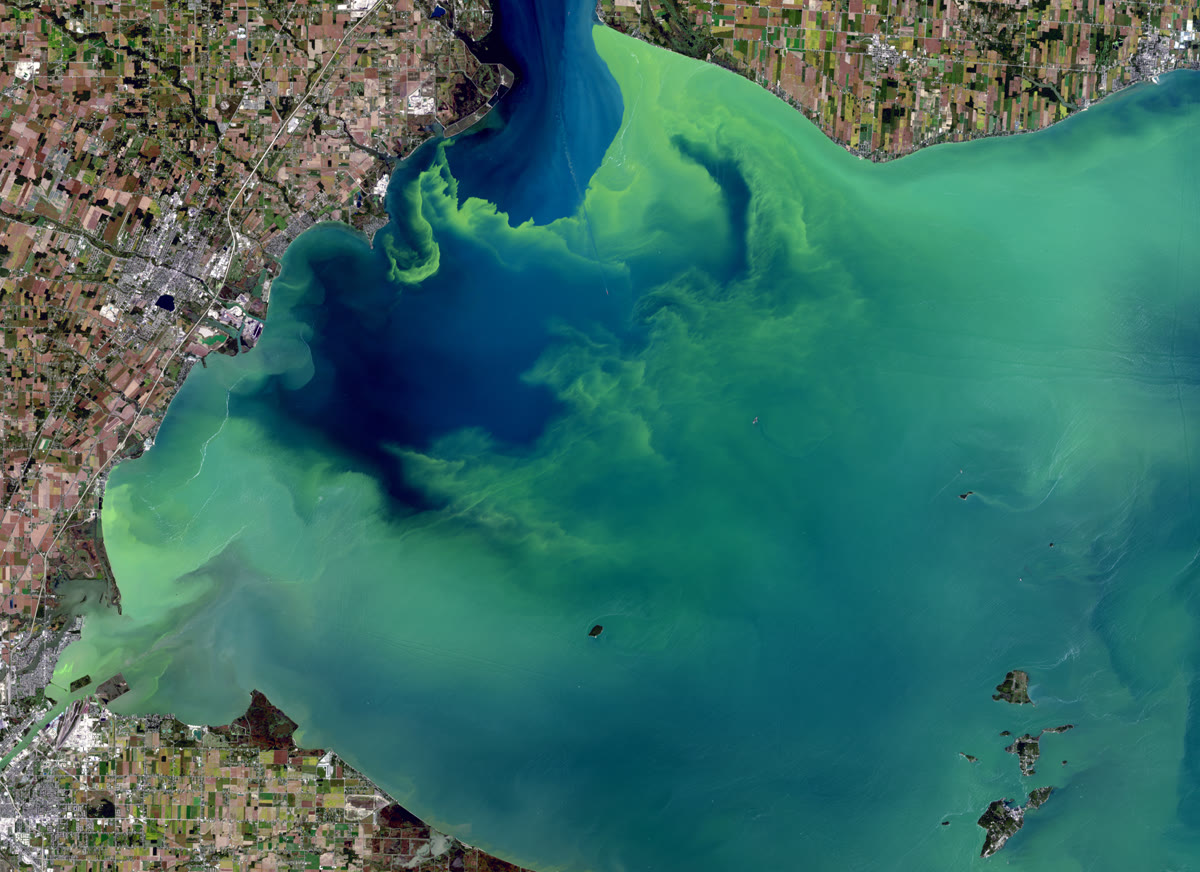
\includegraphics[width=0.62\linewidth]{images/book4/algal-bloom.jpg}

{\small An algal bloom on a large lake, seen by an Earth-observation satellite in
late September: the green swirls are dense populations of microscopic algae
fed by nutrients from the farmland around. Image: USGS and NASA, public domain.}
\end{omfigure}

\section{The atmosphere}

\begin{definition}[Greenhouse gases]\label{def:b3:environmental-toxicology:greenhouse}
A \emph{greenhouse gas}\index{greenhouse gas} absorbs and emits infrared
radiation at the wavelengths of the radiation emitted by the Earth's surface, and
so warms the lower atmosphere. The \emph{global warming
potential}\index{global warming potential} (GWP) of a gas over a time horizon,
usually 100 years, is the energy it traps after the emission of one kilogram,
relative to one kilogram of carbon dioxide.
\end{definition}

A molecule absorbs infrared radiation only through vibrations that change its
dipole moment (\cref{ch:b3:group-theory-applied}). Dinitrogen and dioxygen,
homonuclear diatomics, have no such vibration and are transparent; argon has no
vibration at all. Carbon dioxide, linear and non-polar, has an infrared-active
bending mode near \qty{15}{\micro\metre}, in the middle of the Earth's emission; water, methane
and nitrous oxide absorb at many wavelengths.

% ledger: atm:CO2.2025, atm:CH4.2025, atm:N2O.2025, gwp:CH4.fossil, gwp:CH4.nonfossil, gwp:N2O, life:CH4, life:N2O
In 2025 the global mean mole fractions were \qty{425.6}{ppm} of carbon dioxide, \qty{1936}{ppb} of
methane and \qty{338.9}{ppb} of nitrous oxide. Methane, removed by hydroxyl radicals with a
lifetime of about 12 years, has a GWP-100 of 27 to 30; nitrous oxide, destroyed only in
the stratosphere with a lifetime of about 109 years, of 273. Carbon dioxide has no
single lifetime: part of an emission stays in the air for centuries.

\begin{definition}[Air pollutants]\label{def:b3:environmental-toxicology:pollutants}
\emph{Particulate matter}\index{particulate matter} is the solid and liquid
particles suspended in air, classed by aerodynamic diameter (fine particles
smaller than \qty{2.5}{\micro\metre} reach deep into the lungs). \emph{Acid
rain}\index{acid rain} is rain made more acidic than clean rain by sulfuric and
nitric acids formed from sulfur dioxide and nitrogen oxides.
\end{definition}

\begin{proposition}[pH of clean rain]\label{prop:b3:environmental-toxicology:rain-ph}
Rain in equilibrium with the carbon dioxide of today's air, and with nothing
else, has a pH of about 5.6.
\end{proposition}

\begin{proof}
% ledger: henry:CO2, pka4:H2CO3.1, pkw4:25C, const:atm
Henry's law gives $[\ce{CO2(aq)}] = K_Hp(\ce{CO2}) = \qty{3.4e-7}{mol.L^{-1}.Pa^{-1}} \times (425.6 \times 10^{-6} \times \qty{101325}{Pa}) = \qty{1.47e-5}{mol/L}$. The
charge balance is $[\ce{H+}] = [\ce{HCO3-}] + 2[\ce{CO3^2-}] + [\ce{OH-}] \approx K_{a1}[\ce{CO2(aq)}]/[\ce{H+}] + K_w/[\ce{H+}]$, so
$[\ce{H+}]^2 = K_{a1}[\ce{CO2(aq)}] + K_w = 10^{-6.35} \times \num{1.47e-5} + 10^{-14} = \num{6.6e-12}$: $[\ce{H+}] = \qty{2.6e-6}{mol/L}$, pH 5.6.
\end{proof}

Sulfur dioxide from burning sulfur-containing fuel and nitrogen oxides from
hot combustion are oxidised in the air, by hydroxyl radicals and in cloud
droplets, to sulfuric and nitric acids, which bring rain down to pH 4 and below.
Removing sulfur from fuels and nitrogen oxides from exhausts (catalytic
converters, ammonia injection in power plants) has largely solved the problem
where it was applied. Ozone near the ground, formed when sunlight acts on
nitrogen oxides and volatile organic compounds (\cref{ch:b3:photochemistry}), and
fine particles remain the main air pollutants for health.

\section{Natural waters}

\begin{omfigure}
\begin{tikzpicture}
\begin{axis}[name=a, width=0.48\linewidth, height=5.4cm, xmin=4, xmax=13, ymin=0, ymax=1.02,
  axis lines=left, xlabel={pH}, ylabel={fraction of dissolved carbon},
  tick label style={font=\scriptsize}, label style={font=\small}]
\addplot[color=omDef, thick] table[x=pH, y=a0] {figdata/out/bachelor-3-carbonate-system.dat};
\addplot[color=omMeth, thick] table[x=pH, y=a1] {figdata/out/bachelor-3-carbonate-system.dat};
\addplot[color=omThm, thick] table[x=pH, y=a2] {figdata/out/bachelor-3-carbonate-system.dat};
\node[font=\scriptsize, omDef] at (axis cs:4.9,0.85) {$\ce{CO2(aq)}$};
\node[font=\scriptsize, omMeth] at (axis cs:8.3,0.88) {$\ce{HCO3-}$};
\node[font=\scriptsize, omThm] at (axis cs:12.1,0.85) {$\ce{CO3^2-}$};
\draw[black!30, dashed] (axis cs:6.35,0) -- (axis cs:6.35,0.5) (axis cs:10.33,0) -- (axis cs:10.33,0.5);
\end{axis}
\begin{axis}[at={(a.east)}, anchor=west, xshift=1.4cm, width=0.48\linewidth, height=5.4cm,
  xmin=0, xmax=2000, ymin=5.2, ymax=6.2, axis lines=left,
  xlabel={$\ce{CO2}$ in air / ppm}, ylabel={pH of rain},
  tick label style={font=\scriptsize}, label style={font=\small},
  scaled x ticks=false, xticklabel style={/pgf/number format/1000 sep={}}]
\addplot[color=omDef, thick] table[x=ppm, y=pH] {figdata/out/bachelor-3-carbonate-system-b.dat};
\draw[black!35, dashed] (axis cs:425.6,5.2) -- (axis cs:425.6,5.59);
\node[font=\scriptsize, anchor=west] at (axis cs:470,5.63) {today: 5.6};
\end{axis}
\end{tikzpicture}

{\small Left: distribution of dissolved inorganic carbon among its three forms
against pH at \qty{25}{\celsius}, crossing at $\mathrm pK_{a1} = 6.35$ and $\mathrm pK_{a2} = 10.33$. Right: pH of rain in
equilibrium with carbon dioxide alone, against its mole fraction in air.}
\end{omfigure}

\begin{proposition}[Carbonate fractions]\label{prop:b3:environmental-toxicology:carbonate-fractions}
With $C_T$ the total dissolved inorganic carbon,
$[\ce{CO2(aq)}] = C_Th^2/D$, $[\ce{HCO3-}] = C_TK_{a1}h/D$, $[\ce{CO3^2-}] = C_TK_{a1}K_{a2}/D$, where $h = [\ce{H+}]$ and $D = h^2 + K_{a1}h + K_{a1}K_{a2}$.
\end{proposition}

\begin{proof}
From the two acidity constants,
\[
  [\ce{HCO3-}] = \frac{K_{a1}[\ce{CO2(aq)}]}{h}, \qquad [\ce{CO3^2-}] = \frac{K_{a2}[\ce{HCO3-}]}{h} = \frac{K_{a1}K_{a2}[\ce{CO2(aq)}]}{h^2}.
\]
Their sum is $C_T = [\ce{CO2(aq)}]\,D/h^2$; dividing each form by $C_T$ gives the fractions.
\end{proof}

\begin{definition}[Alkalinity]\label{def:b3:environmental-toxicology:alkalinity}
The \emph{alkalinity}\index{alkalinity} of a water is its capacity to neutralise
strong acid, measured by titration to the end point of carbonic acid (about pH
4.5) and expressed in moles of $\ce{H+}$ per litre.
\end{definition}

\begin{proposition}[Carbonate alkalinity]\label{prop:b3:environmental-toxicology:alkalinity}
In a water whose bases are carbonate species and hydroxide,
$\mathrm{Alk} = [\ce{HCO3-}] + 2[\ce{CO3^2-}] + [\ce{OH-}] - [\ce{H+}]$; it equals the excess of the charges of the strong-base cations
over those of the strong-acid anions, and does not change when carbon dioxide
is exchanged with the air.
\end{proposition}

\begin{proof}
Titration to the carbonic acid end point turns every $\ce{HCO3-}$ into $\ce{CO2}$ (one $\ce{H+}$ each),
every $\ce{CO3^2-}$ into $\ce{CO2}$ (two), every $\ce{OH-}$ into water (one), while the free $\ce{H+}$ already present
counts against: the stated sum. The charge balance of the water, with
$\ce{Na+}$, $\ce{Ca^2+}$\dots{} and $\ce{Cl-}$, $\ce{SO4^2-}$\dots, rearranges to the same sum equal to $\sum z_i c_i$(cations) $-$ $\sum z_jc_j$(anions)
of the strong electrolytes. Adding or removing $\ce{CO2}$ changes none of these ions.
\end{proof}

\begin{definition}[Ocean acidification]\label{def:b3:environmental-toxicology:acidification}
\emph{Ocean acidification}\index{ocean acidification} is the decrease of the
pH of sea water as it takes up carbon dioxide from the air. The \emph{saturation
state}\index{saturation state} of a carbonate mineral is
$\Omega = [\ce{Ca^2+}][\ce{CO3^2-}]/K_{sp}$: above 1 the mineral can form, below 1 it tends to dissolve.
\end{definition}

Dissolved carbon dioxide converts carbonate ions into hydrogencarbonate, $\ce{CO2 + CO3^2- + H2O -> 2HCO3-}$,
lowering the pH and $\Omega$: shells and coral skeletons become harder to build. (In
sea water the constants are apparent ones, measured in the salt medium, and
differ from the fresh-water values of this chapter.)

\begin{definition}[Water hardness]\label{def:b3:environmental-toxicology:hardness}
The \emph{hardness}\index{water hardness} of a water is its total concentration
of calcium and magnesium ions, often expressed as the mass of calcium carbonate
that would contain the same number of moles, in mg/L.
\end{definition}

\begin{definition}[Oxygen demand]\label{def:b3:environmental-toxicology:oxygen-demand}
The \emph{biochemical oxygen demand}\index{biochemical oxygen demand} (BOD) of a
water is the mass of dioxygen consumed per litre by microorganisms oxidising its
organic matter in the dark, over a stated time (five days at \qty{20}{\celsius} for $\mathrm{BOD_5}$). Its
\emph{chemical oxygen demand}\index{chemical oxygen demand} (COD) is the mass of
dioxygen equivalent to the dichromate consumed in oxidising its organic matter
chemically.
\end{definition}

\begin{proposition}[BOD curve]\label{prop:b3:environmental-toxicology:bod}
If biodegradable organic matter is consumed by first-order kinetics with rate
constant $k$, the oxygen used after time $t$ is $\mathrm{BOD}_t = L_0(1 - \eu^{-kt})$, where $L_0$ is the ultimate BOD.
\end{proposition}

\begin{proof}
The remaining demand $L$ obeys $\dd L/\dd t = -kL$, so $L = L_0\eu^{-kt}$; the oxygen used is what has gone,
$L_0 - L$.
\end{proof}

\begin{omfigure}
\begin{tikzpicture}
\begin{axis}[name=a, width=0.48\linewidth, height=5.2cm, xmin=0, xmax=30, ymin=0, ymax=270,
  axis lines=left, xlabel={time / days}, ylabel={BOD / \unit{mg.L^{-1}}},
  tick label style={font=\scriptsize}, label style={font=\small}]
\addplot[color=omDef, thick] table[x=t, y=bod] {figdata/out/bachelor-3-bod.dat};
\draw[black!35, dashed] (axis cs:0,250) -- (axis cs:30,250);
\draw[black!35, dashed] (axis cs:5,0) -- (axis cs:5,170.8);
\node[font=\scriptsize, anchor=west] at (axis cs:5.6,140) {$\mathrm{BOD_5}$};
\node[font=\scriptsize, anchor=north east] at (axis cs:30,246) {$L_0$};
\end{axis}
\begin{axis}[at={(a.east)}, anchor=west, xshift=1.4cm, width=0.48\linewidth, height=5.2cm,
  xmin=0, xmax=15, ymin=0, ymax=10, axis lines=left,
  xlabel={time downstream / days}, ylabel={dissolved $\ce{O2}$ / \unit{mg.L^{-1}}},
  tick label style={font=\scriptsize}, label style={font=\small}]
\addplot[color=omThm, thick] table[x=t, y=O2] {figdata/out/bachelor-3-bod-b.dat};
\draw[black!35, dashed] (axis cs:0,9.1) -- (axis cs:15,9.1);
\node[font=\scriptsize, anchor=south east] at (axis cs:15,9.1) {saturation};
\node[font=\scriptsize, anchor=north] at (axis cs:2.4,6.3) {critical point};
\end{axis}
\end{tikzpicture}

{\small Left: the BOD of a model sewage, $L_0 = \qty{250}{mg/L}$ and $k = \qty{0.23}{d^{-1}}$: about two thirds of the
demand is used in five days. Right: the oxygen sag in a river below an outfall
(Streeter--Phelps model): decay of the organic load consumes oxygen faster than
the air restores it at first, until the deficit peaks after about 2.4 days.}
\end{omfigure}

\begin{method}[Determining the COD]\label{met:b3:environmental-toxicology:cod}
\begin{enumerate}
  \item Reflux a measured volume of sample with a known excess of potassium
        dichromate in sulfuric acid, with silver sulfate as catalyst and
        mercury(II) sulfate to bind chloride.
  \item Titrate the remaining dichromate with iron(II) using ferroin, and run a
        blank with pure water.
  \item The dichromate consumed, converted to the equivalent mass of $\ce{O2}$ (one
        $\ce{Cr2O7^2-}$ takes six electrons, as 1.5 $\ce{O2}$ would), divided by the sample volume, is the
        COD in mg/L.
\end{enumerate}
\end{method}

\begin{definition}[Eutrophication]\label{def:b3:environmental-toxicology:eutrophication}
\emph{Eutrophication}\index{eutrophication} is the enrichment of a water body
with nutrients, chiefly phosphorus and nitrogen, leading to excessive growth of
algae and plants, then to oxygen depletion when they decay.
\end{definition}

\begin{omfigure}
\begin{tikzpicture}[font=\scriptsize, >=Stealth,
  box/.style={draw, rounded corners, align=center, fill=omMeth!10, inner sep=3pt, minimum height=8mm}]
  \node[box] (f) at (-3.4,1.2) {fields: fertiliser,\\ manure};
  \node[box] (t) at (-3.4,-0.4) {towns: sewage,\\ detergents};
  \node[box] (a) at (0,2.1) {atmosphere:\\ deposition (N)};
  \node[box, fill=omDef!12, minimum width=3.2cm, minimum height=1.7cm] (l) at (0.6,0.4) {lake water:\\ algae grow};
  \node[box, fill=black!8] (s) at (0.6,-1.6) {sediment: P stored,\\ released when anoxic};
  \node[box] (o) at (4.0,0.4) {outflow};
  \draw[->, thick] (f) -- node[above, sloped, pos=0.4] {runoff} (l);
  \draw[->, thick] (t) -- node[below, sloped] {N, P} (l);
  \draw[->, thick] (a) -- (l);
  \draw[->, thick] (l) -- node[left] {dead algae} (s);
  \draw[->, thick, dashed] (s.east) to[bend right=30] node[right] {P} (l.south east);
  \draw[->, thick] (l) -- (o);
\end{tikzpicture}

{\small Nutrient flows into and within a lake. Phosphorus, often the limiting
nutrient in fresh water, accumulates in the sediment and returns to the water
when the bottom loses its oxygen, which can sustain blooms for years after the
inputs are cut.}
\end{omfigure}

Algae take up carbon, nitrogen and phosphorus in roughly constant proportions;
whichever nutrient is short relative to those needs limits their growth. In
most lakes it is phosphorus, which is why phosphates were removed from
detergents and from treated sewage; in many coastal seas it is nitrogen.

\begin{definition}[Speciation]\label{def:b3:environmental-toxicology:speciation}
The \emph{chemical speciation}\index{chemical speciation} of an element in a
sample is the distribution of its amount among its chemical forms: oxidation
states, complexes, organometallic compounds, free and bound species.
\end{definition}

Toxicity depends on speciation. Inorganic mercury released into water is
methylated by bacteria in sediments into methylmercury, which crosses membranes,
binds the sulfur of proteins and concentrates up food chains; arsenic is far more
toxic as arsenite, As(III), than as arsenate, As(V), and much less so in the organic
forms found in seafood. A total concentration alone says little.

\begin{method}[Speciation of a metal in a water]\label{met:b3:environmental-toxicology:speciation}
\begin{enumerate}
  \item List the ligands present (hydroxide, carbonate, chloride, sulfate, organic
        matter) with their concentrations and the pH.
  \item Write the complexation constants and the mass balance of the metal, as in the
        Year 1 volume.
  \item Solve for the free metal ion, then each complex; draw the fractions against
        pH or against a ligand concentration.
  \item Compare the toxic or bioavailable form (often the free ion) with the total.
\end{enumerate}
\end{method}

\section{Soils and sediments}

\begin{definition}[Sorption in soils]\label{def:b3:environmental-toxicology:soil}
The \emph{cation exchange capacity}\index{cation exchange capacity} of a soil is
the amount of exchangeable cations it can hold per unit mass, on clays and organic
matter. The \emph{soil--water distribution coefficient}\index{soil--water distribution coefficient}
$K_d$ is the ratio of the concentration of a substance
sorbed on the soil (per kilogram) to its concentration in the pore water (per
litre); the \emph{organic-carbon partition coefficient}\index{organic-carbon partition coefficient}
is $K_{oc} = K_d/f_{oc}$, with $f_{oc}$ the mass fraction of organic carbon.
\end{definition}

Neutral organic compounds sorb mainly on soil organic matter, so that $K_{oc}$ varies
much less from soil to soil than $K_d$. A compound with a small $K_d$ moves with water
and can reach groundwater (leaching); one with a large $K_d$ stays near the surface,
bound to particles that erosion may carry into rivers and lakes.

\section{Fate of pollutants}

\begin{definition}[Octanol--water partition coefficient]\label{def:b3:environmental-toxicology:kow}
The \emph{octanol--water partition coefficient}\index{octanol--water partition coefficient}
$K_{ow}$ of a substance is the ratio of its equilibrium concentrations in
octan-1-ol and in water; it measures its affinity for fatty tissues and organic
matter.
\end{definition}

% ledger: logkow:DDT, logkow:benzene, logkow:atrazine, logkow:PCB153
Benzene has $\log K_{ow} = 2.13$, the herbicide atrazine 2.61, a hexachlorinated PCB 6.67 and
DDT 6.91: the last two dissolve in fat tens of millions of times better than in
water.

\begin{definition}[Bioaccumulation]\label{def:b3:environmental-toxicology:bio}
The \emph{bioconcentration factor}\index{bioconcentration factor} (BCF) is the
ratio of the concentration in an organism to that in the surrounding water at
steady state, uptake from water only. \emph{Bioaccumulation}\index{bioaccumulation}
is the build-up in an organism from all routes, food included;
\emph{biomagnification}\index{biomagnification} is the increase of
concentration from prey to predator up a food chain.
\end{definition}

\begin{proposition}[BCF and $K_{ow}$]\label{prop:b3:environmental-toxicology:bcf-kow}
For neutral organic substances that are not metabolised, $\log\mathrm{BCF}$ in fish is
approximately a linear function of $\log K_{ow}$, with a slope close to 1, up to $\log K_{ow}$ near 6;
above that, uptake slows and the relation levels off (empirical regressions).
\admitted
\end{proposition}

\begin{definition}[Persistent organic pollutants]\label{def:b3:environmental-toxicology:pop}
A \emph{persistent organic pollutant}\index{persistent organic pollutant} is an
organic substance that resists degradation, bioaccumulates, is toxic and is
transported far from its sources, such as DDT, the PCBs and the dioxins.
\end{definition}

\begin{proposition}[Equilibrium distribution between compartments]\label{prop:b3:environmental-toxicology:level-one}
A mass $M$ of a substance distributed at equilibrium (a ``level I'' model) among water
(volume $V_w$), air ($V_a$), sediment solids ($m_s$) and fish ($m_f$) has the water concentration
$C_w = M/(V_w + K_{aw}V_a + K_{sw}m_s + K_{fw}m_f)$, where the $K$ are the partition coefficients relative to
water; the mass in each compartment is its term times $C_w$.
\end{proposition}

\begin{proof}
At equilibrium $C_a = K_{aw}C_w$, $C_s = K_{sw}C_w$ (per kilogram), $C_f = K_{fw}C_w$. The mass balance is
$M = C_wV_w + C_aV_a + C_sm_s + C_fm_f = C_w(V_w + K_{aw}V_a + K_{sw}m_s + K_{fw}m_f)$; dividing gives $C_w$.
\end{proof}

\begin{omfigure}
\begin{tikzpicture}[font=\scriptsize, >=Stealth,
  comp/.style={draw, rounded corners, align=center, minimum width=2.6cm, minimum height=1.0cm}]
  \node[comp, fill=omDef!8] (air) at (0,2.2) {air\\ $C_a = K_{aw}C_w$};
  \node[comp, fill=omDef!25] (w) at (0,0.6) {water\\ $C_w$};
  \node[comp, fill=black!10] (sed) at (0,-1.0) {sediment\\ $C_s = K_{sw}C_w$};
  \node[comp, fill=omMeth!15] (fish) at (3.6,0.6) {fish\\ $C_f = K_{fw}C_w$};
  \node[comp, fill=omProp!15] (soil) at (-3.6,0.6) {soil\\ $C_{soil} = K_dC_w$};
  \draw[<->, thick] (air) -- (w); \draw[<->, thick] (w) -- (sed);
  \draw[<->, thick] (w) -- (fish); \draw[<->, thick] (w) -- (soil);
\end{tikzpicture}

{\small Compartments of an equilibrium (level I) model: every compartment is in
equilibrium with the water, its concentration fixed by a partition coefficient.
The substance accumulates where the product of capacity and volume (or mass) is
largest, often the sediment or soil for a hydrophobic compound.}
\end{omfigure}

\section{Toxicology and regulation}

\begin{definition}[Dose--response]\label{def:b3:environmental-toxicology:dose}
A \emph{dose--response relationship}\index{dose--response relationship} links
the dose of a substance to the size or frequency of an effect. The \emph{median
lethal dose}\index{median lethal dose} $\mathrm{LD_{50}}$ kills half of a test population; the
\emph{median effective concentration}\index{median effective concentration} $\mathrm{EC_{50}}$
causes a stated effect in half. The \emph{no-observed-adverse-effect
level}\index{no-observed-adverse-effect level} (NOAEL) is the highest tested dose
without an adverse effect, the \emph{lowest-observed-adverse-effect
level}\index{lowest-observed-adverse-effect level} (LOAEL) the lowest tested dose
with one.
\end{definition}

\begin{proposition}[Log-logistic model]\label{prop:b3:environmental-toxicology:dose-response}
In the log-logistic model $f(d) = 1/\bigl(1 + (D_{50}/d)^n\bigr)$, the response is one half at $d = D_{50}$, and $n$
measures the steepness: the dose ratio between 10\,\% and 90\,\% responses is $81^{1/n}$.
\end{proposition}

\begin{proof}
At $d = D_{50}$, $f = 1/2$. $f = 0.1$ requires $(D_{50}/d)^n = 9$, $f = 0.9$ requires $(D_{50}/d)^n = 1/9$; the ratio of the two doses
is $(9 \times 9)^{1/n} = 81^{1/n}$.
\end{proof}

\begin{omfigure}
\begin{tikzpicture}
\begin{axis}[width=0.72\linewidth, height=5.4cm, xmode=log, xmin=3, xmax=3200, ymin=0, ymax=1.02,
  axis lines=left, xlabel={dose / \unit{mg.kg^{-1}}}, ylabel={fraction responding},
  tick label style={font=\scriptsize}, label style={font=\small}]
\addplot[color=omDef, thick] table[x=d, y=n2] {figdata/out/bachelor-3-dose-response.dat};
\addplot[color=omThm, thick] table[x=d, y=n6] {figdata/out/bachelor-3-dose-response.dat};
\addplot[only marks, mark=*, mark size=1.6pt, omThm] table[x=d, y=r] {figdata/out/bachelor-3-dose-response-b.dat};
\draw[black!35, dashed] (axis cs:200,0) -- (axis cs:200,0.5) -- (axis cs:3,0.5);
\node[font=\scriptsize, anchor=north west] at (axis cs:200,0.48) {$D_{50}$};
\node[font=\scriptsize, omThm, anchor=south east, inner sep=1pt] (noael) at (axis cs:60,0.09) {NOAEL};
\draw[omThm] (noael.south east) -- (axis cs:78,0.012);
\node[font=\scriptsize, omThm, anchor=west] at (axis cs:165,0.2) {LOAEL};
\node[font=\scriptsize, omDef, anchor=east] at (axis cs:60,0.25) {$n = 2$};
\node[font=\scriptsize, omThm, anchor=east] at (axis cs:185,0.8) {$n = 6$};
\end{axis}
\end{tikzpicture}

{\small Log-logistic dose--response curves with the same median dose (\qty{200}{mg/kg},
model) and two steepnesses. The dots are a study at five doses for the steeper
curve: with a 5\,\% response as the criterion of an adverse effect, the NOAEL is
\qty{80}{mg/kg} and the LOAEL \qty{160}{mg/kg}; both depend on the doses chosen.}
\end{omfigure}

\begin{definition}[Acute and chronic toxicity]\label{def:b3:environmental-toxicology:toxicity}
\emph{Acute toxicity}\index{acute toxicity} is the harm caused by a single
exposure or exposures within a short time; \emph{chronic toxicity}\index{chronic toxicity},
by repeated or continuous exposure over a long part of a lifetime.
\end{definition}

% ledger: ld50:NaCl, ld50:caffeine, ld50:nicotine
Toxicity is a matter of dose: the oral $\mathrm{LD_{50}}$ in rats is about \qty{3000}{mg/kg} for sodium chloride,
\qty{192}{mg/kg} for caffeine and \qty{188}{mg/kg} for nicotine in the same kind of record. For most effects a
threshold dose exists below which the body copes; for genotoxic carcinogens
none is assumed, and exposure is kept as low as reasonably achievable.

\begin{definition}[Ecotoxicology]\label{def:b3:environmental-toxicology:ecotoxicology}
\emph{Ecotoxicology}\index{ecotoxicology} studies the effects of substances on
organisms in ecosystems. The \emph{predicted no-effect
concentration}\index{predicted no-effect concentration} (PNEC) is the lowest
effect or no-effect concentration from tests on representative species,
divided by an assessment factor that covers the uncertainty; the
\emph{predicted environmental concentration}\index{predicted environmental concentration}
(PEC) is the concentration expected from the uses and fate of the
substance; the \emph{risk quotient}\index{risk quotient} is PEC/PNEC.
\end{definition}

\begin{proposition}[Risk quotient]\label{prop:b3:environmental-toxicology:risk-quotient}
A \omterm{def:b3:environmental-toxicology:ecotoxicology}{risk quotient} below 1 indicates no concern for the compartment assessed; above
1, a risk that calls for refined data or measures to reduce exposure.
\end{proposition}

\begin{proof}[By definition]
The PNEC is set, through its assessment factor, below the concentrations at which
effects were seen; an expected concentration below it is therefore not
expected to cause effects, and above it is.
\end{proof}

\begin{method}[An environmental risk assessment]\label{met:b3:environmental-toxicology:risk}
\begin{enumerate}
  \item Hazard: collect toxicity data for algae, invertebrates and fish (acute
        $\mathrm{EC_{50}}$, chronic NOEC); take the lowest; divide by the assessment factor (larger when
        only acute data exist) to get the PNEC.
  \item Exposure: from the amounts used and the fate (partitioning, degradation),
        compute the PEC in each compartment, or measure it.
  \item Risk: compute PEC/PNEC; if above 1, refine the data or reduce the
        exposure, and repeat.
\end{enumerate}
\end{method}

\begin{definition}[Occupational exposure limit]\label{def:b3:environmental-toxicology:oel}
An \emph{occupational exposure limit}\index{occupational exposure limit} is the
concentration of a substance in the air of a workplace that workers may breathe,
averaged over a working day (or over 15 minutes for short-term limits), without
expected adverse effects.
\end{definition}

New chemicals placed on a market in quantity must be registered with a
dossier of their properties, hazards and uses; the most hazardous may be
restricted or allowed only for authorised uses.

\begin{inthelab}[Measuring $\mathrm{BOD_5}$]
A sample is diluted with aerated dilution water containing nutrients and a
bacterial seed, so that a good part, but not all, of the oxygen will be consumed. Two
stoppered bottles are filled to the brim: the dissolved oxygen of one is measured
at once with an oxygen electrode, the other after five days in the dark at
\qty{20}{\celsius}. The difference, times the dilution factor and corrected for the seed, is the
$\mathrm{BOD_5}$.
\end{inthelab}

\begin{safety}{\ghs[0.62cm]{GHS03}\ghs[0.62cm]{GHS05}\ghs[0.62cm]{GHS06}\ghs[0.62cm]{GHS08}\ghs[0.62cm]{GHS09}}
% ledger: ghs:K2Cr2O7, ghs4:HgSO4
The COD reagents: potassium dichromate is an oxidiser, may cause cancer and
genetic defects, is corrosive and sensitising; mercury(II) sulfate is fatal if
swallowed, inhaled or in contact with skin and very toxic to aquatic life. Both are
used in sealed tubes, and the spent tubes go to hazardous waste.
\end{safety}

\begin{history}[A book and a bay]
In 1962 Rachel Carson's \textit{Silent Spring} described the decline of birds poisoned by
DDT and other pesticides concentrated up food chains, and launched modern
environmental regulation. A few years earlier, in 1956, a disease of the nervous
system was recognised among the people of Minamata Bay: a chemical plant had
discharged methylmercury, formed from its mercury catalyst, which accumulated
in the fish the inhabitants ate.
\end{history}

\section{Exercises}

\begin{exercise}[$\star$]\label{exo:b3:environmental-toxicology:1}
Why do $\ce{N2}$, $\ce{O2}$ and Ar not absorb in the infrared, and which vibration of $\ce{CO2}$ makes it a
\omterm{def:b3:environmental-toxicology:greenhouse}{greenhouse gas}?
\end{exercise}

\begin{exercise}[$\star$]\label{exo:b3:environmental-toxicology:2}
By what factor does $[\ce{H+}]$ change when the pH of sea water falls by 0.1?
\end{exercise}

\begin{exercise}[$\star$]\label{exo:b3:environmental-toxicology:3}
A water contains \qty{2.0}{mmol/L} of $\ce{Ca^2+}$ and \qty{0.50}{mmol/L} of $\ce{Mg^2+}$. Give its \omterm{def:b3:environmental-toxicology:hardness}{hardness} in mg of $\ce{CaCO3}$ per litre.
\end{exercise}

\begin{exercise}[$\star$]\label{exo:b3:environmental-toxicology:4}
Algae take up C, N and P in the mole ratio $106 : 16 : 1$ (data of the exercise). A lake water
has \qty{0.60}{mg/L} of nitrate nitrogen and \qty{0.010}{mg/L} of phosphate phosphorus. Which nutrient limits
growth?
\end{exercise}

\begin{exercise}[$\star\star$]\label{exo:b3:environmental-toxicology:5}
A $\mathrm{BOD_5}$ of \qty{170}{mg/L} is measured on a sewage with $k = \qty{0.23}{d^{-1}}$. Estimate its ultimate BOD.
\end{exercise}

\begin{exercise}[$\star\star$]\label{exo:b3:environmental-toxicology:6}
A \qty{100.0}{mL} water sample needs \qty{4.40}{mL} of \qty{0.0200}{mol/L} hydrochloric acid to reach pH 4.5. Compute its
\omterm{def:b3:environmental-toxicology:alkalinity}{alkalinity} and, assuming it is all hydrogencarbonate, its concentration in mg/L.
\end{exercise}

\begin{exercise}[$\star\star$]\label{exo:b3:environmental-toxicology:7}
A soil has $f_{oc} = 0.020$; a pesticide has $K_{oc} = \qty{300}{L/kg}$ (data of the exercise). Compute $K_d$ and the
fraction of the pesticide sorbed in a soil with \qty{1.5}{kg} of solid per \qty{0.30}{L} of pore water.
\end{exercise}

\begin{exercise}[$\star\star$]\label{exo:b3:environmental-toxicology:8}
With $\log\mathrm{BCF} = 0.85\log K_{ow} - 0.70$ (an empirical regression, data of the exercise), estimate the BCF of
benzene and of a hexachlorinated PCB, and comment.
\end{exercise}

\begin{exercise}[$\star\star$]\label{exo:b3:environmental-toxicology:9}
Express the rat oral $\mathrm{LD_{50}}$ of caffeine as a mass for a \qty{70}{kg} adult and as cups of coffee of
\qty{90}{mg} each (a naive scaling, data of the exercise). Why is such a scaling only indicative?
\end{exercise}

\begin{exercise}[$\star\star\star$]\label{exo:b3:environmental-toxicology:10}
A substance has a 48-hour $\mathrm{EC_{50}}$ of \qty{0.50}{mg/L} for water fleas, a 72-hour $\mathrm{EC_{50}}$ of \qty{1.2}{mg/L} for algae
and a 96-hour $\mathrm{LC_{50}}$ of \qty{2.0}{mg/L} for fish, all acute, and an assessment factor of 1000 applies
(data of the exercise). Compute the PNEC, and the \omterm{def:b3:environmental-toxicology:ecotoxicology}{risk quotient} for a PEC of \qty{0.20}{\micro g/L}.
\end{exercise}

\begin{exercise}[$\star\star\star$]\label{exo:b3:environmental-toxicology:11}
A fish-eating bird eats fish with \qty{0.30}{mg/kg} of a persistent pollutant; the fish eat
plankton with \qty{0.015}{mg/kg}; the water contains \qty{2.0}{ng/L}. Compute the bioconcentration and
\omterm{def:b3:environmental-toxicology:bio}{biomagnification} factors along the chain if the bird's fat holds \qty{6.0}{mg/kg} (data of the
exercise).
\end{exercise}

\begin{exercise}[$\star\star\star$]\label{exo:b3:environmental-toxicology:12}
A power plant emits \qty{1000}{t} of $\ce{SO2}$ a year. Compute the mass of sulfuric acid it can make,
and the volume of rain it would bring to pH 4.0 if all of it fell in rain (ignore other
acids and bases).
\end{exercise}

\section{Problem: A Pesticide in a Lake}

\begin{problem}[{Weekend problem --- a pesticide in a lake: its partitioning into
sediment and fish, an equilibrium mass balance, its degradation over a year,
and the risk quotient for the lake's organisms}]
\label{pb:b3:environmental-toxicology:1}
Data of the problem. A lake holds $\qty{1.0e9}{L}$ of water under $\qty{1.0e12}{L}$ of air (the mixed layer above it),
with $\qty{1.0e8}{kg}$ of active sediment solids ($f_{oc} = 0.040$) and $\qty{1.0e4}{kg}$ of fish (lipid fraction 0.048).
A pesticide has $\log K_{ow} = 4.0$, an air--water partition coefficient $K_{aw} = \num{1.0e-4}$, and $K_{oc} = 0.41\,K_{ow}$;
$K_{fw}$ = lipid fraction $\times K_{ow}$. 100 kg of it reach the lake. Its half-life in the lake is 60 days.
The most sensitive chronic test gives a NOEC of \qty{50}{\micro g/L}, with an assessment factor of 10;
fish for human consumption should not exceed \qty{1.0}{mg/kg}.

\medskip\noindent\textbf{Part I --- Partition coefficients.}
\begin{enumerate}
  \item What does $\log K_{ow} = 4.0$ say about the pesticide?
  \item Compute $K_{oc}$ and the sediment--water coefficient $K_{sw}$.
  \item Compute the fish--water coefficient $K_{fw}$.
  \item Is the pesticide volatile from water? Use $K_{aw}$.
  \item Why does organic carbon, not mineral matter, govern its sorption?
  \item Which compartment do you expect to hold most of it?
\end{enumerate}

\medskip\noindent\textbf{Part II --- Equilibrium mass balance.}
\begin{enumerate}[resume]
  \item Compute the capacity terms $V_w$, $K_{aw}V_a$, $K_{sw}m_s$ and $K_{fw}m_f$.
  \item Compute the water concentration.
  \item Compute the mass in each compartment.
  \item Compute the concentrations in air, sediment and fish.
  \item Which assumption of the model is least realistic?
  \item How would degradation change the picture (level II and III models)?
\end{enumerate}

\medskip\noindent\textbf{Part III --- Degradation.}
\begin{enumerate}[resume]
  \item Compute the first-order rate constant.
  \item Compute the fraction left after one year.
  \item Compute the water concentration after one year.
  \item Why may the sediment hold the pesticide longer than the half-life suggests?
  \item What makes a pesticide persistent?
\end{enumerate}

\medskip\noindent\textbf{Part IV --- Risk.}
\begin{enumerate}[resume]
  \item Compute the PNEC.
  \item Take the initial water concentration as PEC: compute the \omterm{def:b3:environmental-toxicology:ecotoxicology}{risk quotient}.
  \item Conclude for the lake's organisms.
  \item Compare the fish concentration with the consumption threshold.
  \item What would you measure next, and where?
  \item Which measures would lower the PEC?
  \item Why does the assessment factor matter so much?
  \item State the result: the \omterm{def:b3:environmental-toxicology:ecotoxicology}{risk quotient} PEC/PNEC.
\end{enumerate}
\end{problem}
